\documentclass[11pt,a4paper]{report}%especifica o tipo de documento que tenciona escrever: carta, artigo, relatório... neste caso é um relatório
% [11pt,a4paper] Define o tamanho principal das letras do documento. caso não especifique uma delas, é assumido 10pt
% a4paper -- Define o tamanho do papel.
\usepackage{subcaption}

\usepackage[portuges]{babel}%Babel -- irá activar automaticamente as regras apropriadas de hifenização para a língua todo o
                                   %-- o texto gerado é automaticamente traduzido para Português.
                                   %  Por exemplo, “chapter” irá passar a “capítulo”, “table of contents” a “conteúdo”.
                                   % portuges -- específica para o Português.
\usepackage[utf8]{inputenc} % define o encoding usado texto fonte (input)--usual "utf8" ou "latin1

\usepackage{graphicx} %permite incluir graficos, tabelas, figuras
\usepackage{url} % para utilizar o comando \url{}
\usepackage{enumerate} %permite escolher, nas listas enumeradas, se os iems sao marcados com letras ou numeros-romanos em vez de numeracao normal

%\usepackage{apalike} % gerar biliografia no estilo 'named' (apalike)

\usepackage{color} % Para escrever em cores

\usepackage{multirow} %tabelas com multilinhas
\usepackage{array} %formatação especial de tabelas em array

\usepackage[pdftex]{hyperref} % transformar as referências internas do seu documento em hiper-ligações.

%Exemplos de fontes -- nao e vulgar mudar o tipo de fonte
%\usepackage{tgbonum} % Fonte de letra: TEX Gyre Bonum
%\usepackage{lmodern} % Fonte de letra: Latin Modern Sans Serif
%\usepackage{helvet}  % Fonte de letra: Helvetica
%\usepackage{charter} % Fonte de letra:Charter

\definecolor{saddlebrown}{rgb}{0.55, 0.27, 0.07} % para definir uma nova cor, neste caso 'saddlebrown'

\usepackage{listings}  % para utilizar blocos de texto verbatim no estilo 'listings'
%paramerização mais vulgar dos blocos LISTING - GENERAL
\lstset{
	basicstyle=\small, %o tamanho das fontes que são usadas para o código
	numbers=left, % onde colocar a numeração da linha
	numberstyle=\tiny, %o tamanho das fontes que são usadas para a numeração da linha
	numbersep=5pt, %distancia entre a numeração da linha e o codigo
	breaklines=true, %define quebra automática de linha
    frame=tB,  % caixa a volta do codigo
	mathescape=true, %habilita o modo matemático
	escapeinside={(*@}{@*)} % se escrever isto  aceita tudo o que esta dentro das marcas e nao altera
}
%
%\lstset{ %
%	language=Java,							% choose the language of the code
%	basicstyle=\ttfamily\footnotesize,		% the size of the fonts that are used for the code
%	keywordstyle=\bfseries,					% set the keyword style
%	%numbers=left,							% where to put the line-numbers
%	numberstyle=\scriptsize,				% the size of the fonts that are used for the line-numbers
%	stepnumber=2,							% the step between two line-numbers. If it's 1 each line
%											% will be numbered
%	numbersep=5pt,							% how far the line-numbers are from the code
%	backgroundcolor=\color{white},			% choose the background color. You must add \usepackage{color}
%	showspaces=false,						% show spaces adding particular underscores
%	showstringspaces=false,					% underline spaces within strings
%	showtabs=false,							% show tabs within strings adding particular underscores
%	frame=none,								% adds a frame around the code
%	%abovecaptionskip=-.8em,
%	%belowcaptionskip=.7em,
%	tabsize=2,								% sets default tabsize to 2 spaces
%	captionpos=b,							% sets the caption-position to bottom
%	breaklines=true,						% sets automatic line breaking
%	breakatwhitespace=false,				% sets if automatic breaks should only happen at whitespace
%	title=\lstname,							% show the filename of files included with \lstinputlisting;
%											% also try caption instead of title
%	escapeinside={\%*}{*)},					% if you want to add a comment within your code
%	morekeywords={*,...}					% if you want to add more keywords to the set
%}

\usepackage{xspace} % deteta se a seguir a palavra tem uma palavra ou um sinal de pontuaçao se tiver uma palavra da espaço, se for um sinal de pontuaçao nao da espaço

\parindent=0pt %espaço a deixar para fazer a  indentação da primeira linha após um parágrafo
\parskip=2pt % espaço entre o parágrafo e o texto anterior

\setlength{\oddsidemargin}{-1cm} %espaço entre o texto e a margem
\setlength{\textwidth}{18cm} %Comprimento do texto na pagina
\setlength{\headsep}{-1cm} %espaço entre o texto e o cabeçalho
\setlength{\textheight}{23cm} %altura do texto na pagina

% comando '\def' usado para definir abreviatura (macros)
% o primeiro argumento é o nome do novo comando e o segundo entre chavetas é o texto original, ou sequência de controle, para que expande
\def\darius{\textsf{Darius}\xspace}
\def\antlr{\texttt{AnTLR}\xspace}
\def\pe{\emph{Processamento de Linguagens}\xspace}
\def\titulo#1{\section{#1}}    %no corpo do documento usa-se na forma '\titulo{MEU TITULO}'
\def\super#1{{\em Supervisor: #1}\\ }
\def\area#1{{\em \'{A}rea: #1}\\[0.2cm]}
\def\resumo{\underline{Resumo}:\\ }

%\input{LPgeneralDefintions} %permite ler de um ficheiro de texto externo mais definições

\title{Processamento de Linguagens\\
       \textbf{Trabalho Prático Grupo 6 "AAAAAA"}\\ Relatório de Desenvolvimento
       } %Titulo do documento
%\title{Um Exemplo de Artigo em \LaTeX}
\author{Francisca Barros\\ (a96434) \and Joana Pereira\\ (a97588)
         \and Rafael Correia\\ (a94870)
       } %autores do documento
\date{\today} %data

\begin{document} % corpo do documento
\maketitle % apresentar titulo, autor e data

\begin{abstract}  % resumo do documento


O presente relatório descreve o trabalho prático realizado pelo Grupo 6 no âmbito da Unidade Curricular de Processamento de Linguagens. O objetivo do trabalho foi desenvolver um conversor de \textit{Pug} para \textit{HTML}, utilizando os componentes \textit{Lexer} e \textit{Yacc} para realizar a análise léxica e sintática do código \textit{Pug}. O grupo procurou implementar as funcionalidades necessárias para a maioria dos casos de ficheiros \textit{Pug}, explorando as características da linguagem, como atributos, condicionais, iterações, entre outros. Ao longo do processo de implementação e testes, os resultados obtidos demonstraram a capacidade do conversor em converter corretamente o código \textit{Pug} para \textit{HTML}, preservando a estrutura e o conteúdo dos ficheiros.
\end{abstract}

\tableofcontents % Insere a tabela de indice
%\listoffigures % Insere a tabela de indice figuras
%\listoftables % Insere a tabela de indice tabelas

\chapter{Introdução} \label{chap:intro} %referência cruzada


\titulo{Um belo Projeto}
O presente relatório descreve o trabalho prático realizado pelo Grupo 6 no âmbito da Unidade Curricular de Processamento de Linguagens, inserida no curso de Licenciatura em Engenharia Informática durante o 2º Semestre do ano letivo 2022/2023.

Neste projeto, o grupo optou por abordar o tema 2.5, que consiste na criação de um conversor de \textit{Pug} para \textit{HTML}. O \textit{Pug} é uma linguagem de modelação de \textit{templates} para \textit{Node.js}, reconhecida pela sua sintaxe simples e intuitiva. A escolha deste tema revelou-se interessante para o grupo devido à familiaridade com essa linguagem, adquirida na disciplina de Engenharia Web.

O objetivo deste trabalho é desenvolver um conversor de \textit{Pug} para \textit{HTML}, capaz de implementar as funcionalidades necessárias para a maioria dos casos de ficheiros \textit{Pug}. Procurámos criar um conversor que seja eficiente e capaz de preservar corretamente a estrutura e o conteúdo dos ficheiros, garantindo a correta conversão para o formato \textit{HTML}.

O relatório está dividido em várias secções. Iniciamos com a introdução, que apresenta uma visão geral do trabalho realizado. Em seguida, abordamos a análise e especificação, onde descrevemos informalmente o problema a ser resolvido e estabelecemos os requisitos necessários para a sua resolução. Posteriormente, apresentamos a conceção/desenho da solução, detalhando as estratégias adotadas para o desenvolvimento do conversor. Prosseguimos com a secção de codificação e testes, onde descrevemos o processo de implementação e os testes realizados para verificar a correta funcionalidade do conversor. Por fim, concluímos o relatório com uma síntese das principais conclusões obtidas ao longo do projeto.

O objetivo final deste trabalho é fornecer um conversor de \textit{Pug} para \textit{HTML} que atenda aos requisitos estabelecidos, permitindo a correta conversão de ficheiros \textit{Pug} em \textit{HTML} de forma eficiente e confiável.
\newpage


\chapter{Análise e Especificação} \label{chap:analiseEspecificacao} %capitulo e referencia cruzada
\section{Descrição informal do problema} \label{sec:descricaoProblema} %seccao e referencia cruzada
O objetivo deste projeto é criar um conversor de ficheiros \textit{.pug} para ficheiros \textit{.html}, garantindo a preservação correta de toda a informação. Em outras palavras, ao utilizar um ficheiro em qualquer um dos formatos, não deverá haver diferenças visuais. Para atingir este objetivo, iremos utilizar a biblioteca \cite{PLY}, criando \textit{tokens} com o \textit{ply.lexer} e um \textit{parser} com o \textit{ply.yacc}. O nosso foco é assegurar a conversão adequada entre os formatos, mantendo a integridade dos elementos e a formatação correta, de modo a proporcionar um resultado consistente e de qualidade.


\section{Especificação dos Requisitos}
Como requisitos iniciais do nosso projeto, definimos as funcionalidades necessárias para ser possível converter o exemplo fornecido pelo professor. Após obtermos sucesso nessa etapa, avançamos para a implementação das várias funcionalidades extra do \textit{Pug}. Para isso, consultámos a documentação do \cite{Pug} e dedicámo-nos a incorporar cada uma das suas características no nosso conversor de \textit{Pug} para \textit{HTML}. Sendo estas:

\begin{itemize}
    \item Atributos: Implementar a capacidade de lidar com atributos em várias linhas, entre aspas, com interpolação, booleanos e de estilo.
    \item Condicionais: Desenvolver a funcionalidade de condicionais, como o \textit{if}, \textit{else if}, \textit{else} e \textit{unless} permitindo controlar o fluxo do programa com base em determinadas condições.
    \item Iterações: Implementar iterações utilizando estruturas como \textit{each} e \textit{while}, permitindo repetir blocos de código com base em listas ou condições. Dessa forma, garantimos a correta renderização e repetição dos elementos no ficheiro \textit{HTML}.
    \item Interpolação: Desenvolver a funcionalidade de interpolação, permitindo a inserção de variáveis ou expressões dentro do próprio texto. Isso possibilita a correta substituição e exibição dos valores no ficheiro \textit{HTML} final.
    \item Herança de \textit{templates}: Implementar a capacidade de herança de \textit{templates}, permitindo a criação de \textit{layouts} ou estruturas comuns que podem ser estendidos por outros ficheiros \textit{Pug}. Isso garante a correta organização e reutilização de código no processo de conversão para \textit{HTML}.
    \item \textit{Mixins}: Desenvolver a funcionalidade de \textit{mixins}, que são blocos de código reutilizáveis, permitindo a definição e invocação de trechos de código em diferentes partes de um ficheiro \textit{Pug}. Isso proporciona uma maior modularidade e reutilização de código no processo de conversão.
    \item Texto simples: Implementar a capacidade de incluir texto simples, sem qualquer marcação específica. Dessa forma, garantimos a correta representação do texto no ficheiro \textit{HTML} gerado.
    \item \textit{Tags}: Desenvolver uma sintaxe simplificada para a criação de \textit{tags} \textit{HTML}, facilitando a estruturação e formatação do documento final. Isso garante a correta conversão das \textit{tags} para o formato \textit{HTML} correspondente.
\end{itemize}

Ao abordarmos cada uma dessas características, procuramos implementá-las adequadamente no nosso conversor de \textit{Pug} para \textit{HTML}, garantindo a correta conversão e preservação dos elementos e estruturas no ficheiro \textit{HTML} gerado. Dessa forma, buscamos entregar um conversor funcional e eficiente, capaz de lidar com diversas funcionalidades do \textit{Pug} e produzir resultados de alta qualidade.


\chapter{Concepção/desenho da Resolução}

No Capítulo 3, intitulado "Conceção/Desenho da Resolução", iremos abordar a fase de conceção e desenho da solução para o desenvolvimento do conversor de \textit{Pug} para \textit{HTML}. Nesta etapa, iremos explorar dois componentes essenciais: o \textit{Lexer} (Analisador Léxico) e o \textit{Parser} (Analisador Sintático). O \textit{Lexer} será responsável por realizar a análise léxica do código fonte em \textit{Pug}, identificando os diferentes \textit{tokens} presentes no ficheiro. Já o \textit{Parser} irá realizar a análise sintática, definindo a estrutura gramatical do código \textit{Pug} e permitindo a construção do código HTML correspondente. Através da exploração destes componentes, iremos estabelecer as bases para a implementação eficiente e correta do conversor.

No nosso conversor de \textit{Pug} para \textit{HTML}, conseguimos implementar várias funcionalidades essenciais do \textit{Pug}, enriquecendo a conversão de código de forma significativa. Estas são:
\begin{itemize}
    \item Atributos e Atributos em multiplas linhas
    \item \textit{Class Literal}: Implementamos a capacidade de utilizar a sintaxe do \textit{Pug} para definir classes diretamente nos elementos \textit{HTML}, facilitando a atribuição de estilos e seleção de elementos e evitando a constante definição de \textit{tags div}.
    \item \textit{ID Literal}: Da mesma forma, também permitimos a utilização de IDs literais nos elementos HTML, permitindo a identificação única de elementos específicos no código convertido.
    \item Declaração de variáveis: Além disso, o nosso conversor é capaz de lidar com declarações de variáveis (ex: var x = 0).
    \item Comentários: Implementamos o suporte para a maioria dos tipos de comentários disponíveis no \textit{Pug}, permitindo a inclusão de notas e observações no código.
    \item Condicionais: Conseguímos interpretar e converter condicionais do Pug (\textit{if,else if,else, unless}), possibilitando a execução condicional de trechos de código HTML com base em certas condições lógicas.
    \item \textit{DOCTYPES}: Também conseguimos implementar o suporte aos diferentes tipos de \textit{DOCTYPES} disponíveis no \textit{Pug}, permitindo especificar a versão e o tipo de documento HTML gerado.
    \item \textit{Includes} em \textit{Plain Text}: com esta funcionalidade conseguímos implementar no ficheiro \textit{Pug} textos contidos noutros ficheiros de texto.
    \item Interpolação de Variáveis - é possível substituir variáveis em condições ou em tags seguidas de um igual (ex: title= pageTitle).
    \item Iterações: Implementámos o \textit{while} e o \textit{each}, permitindo a repetição de blocos de código HTML com base em determinadas condições ou listas de dados.
    \item Texto simples
\end{itemize}

\section{Lexer}

Para o \textit{Lexer} fomos definindo os \textit{tokens} de acordo com as funcionalidades que íamos acrescentando e estão divididos em 3 tipos: \textit{literals}, \textit{reserved} e \textit{tokens}.

Os \textit{literals}, tal como é referido na documentação do \cite{PLY}, é definido por: \textit{"simply a single character that is returned "as is" when encountered by the lexer. Literals are checked after all of the defined regular expression rules."}. Nós definimos como sendo:
\begin{verbatim}
literals = [',', ':','[',']','{','}','=']
\end{verbatim}

Os \textit{reserved}, também referidos na documentação, são um dicionário que associa palavras reservadas ao respetivo \textit{token}. 
\begin{verbatim}
reserved = {
   'if' : 'IF',
   'else' : 'ELSE',
   'while' : 'WHILE',
   'unless' : 'UNLESS',
   'each':'EACH',
   'in':'IN',
   'include':'INCLUDE'
}
\end{verbatim}

Finalmente, os restantes \textit{tokens} são definidos numa lista, posteriormente adicionada aos \textit{tokens reserved}.

\begin{verbatim}
    tokens = [
    'POINT',
    'PA',
    'PF',
    'EQUALS',
    'TAG',
    'ID',
    'CLASS',
    'ATTRIBUTE',
    'TEXT',
    'NEWLINE',
    'INDENT',
    'DEDENT',
    'CONDITION',
    'LINECOMMENT',
    'BLOCKCOMMENT',
    'PIPED',
    'VALUE',
    'IGNORE_BLOCKCOMMENT',
    'IGNORE_LINECOMMENT',
    'COMMENT',
    'HASHTAG',
    'NUMBER',
    'STRING',
    'JS',
    'VAR'
] + list(reserved.values())
\end{verbatim}

Cada token tem associado uma função especifica, no nosso caso, a função mais complexa acaba por ser a função que deteta \textit{newlines}, visto que é quando aparece uma nova linha que normalmente se muda de estado. Esta função calcula a nova identação comparando-a com a antiga. Consoante o resultado, e o estado em que estamos, são feitas ações diferentes, como vai ser falado posteriormente.

Além dos \textit{tokens}, foram também definidos vários estados para permitir a identificação dos diferentes \textit{tokens} corretamente. %explicar melhor isto?

\begin{verbatim}
    states = (
    ('comment', 'exclusive'),
    ('ignoreComments', 'exclusive'),
    ('dedent','exclusive'),
    ('indent','exclusive'),
    ('firstWord', 'inclusive'),
    ('pointState', 'exclusive'),
    ('conditional', 'exclusive'),
    ('each', 'exclusive'),
    ('js','exclusive')
    
)



\end{verbatim}



\subsection{Estados comment e ignoreComments}

Ambos os estados servem para idenficar comentários em bloco. Quando é detetado um "//" ou um "//-" com espaços no resto da linha entra-se no estado comment ou ignoreComments, dependendo do que é detetado. Estando neste estado, e visto que a função é exclusiva, existem apenas uma forma de sair do estado, através da função que lê new lines, visto que esta está declarada para todos os estados:

\begin{verbatim}
    def t_ANY_newline(t)
\end{verbatim}

Assim, ambos os estados são acabados quando é reconhecido um DEDENT (uma diminuição de identação).


\subsection{Estados dedent e indent}

Estes estados são usados para criar os tokens INDENT e DEDENT. Quando o lexer entra na função do newline, verifica se a identação mudou e consoante a mudança muda uma variável que indica o número de tokens INDENT/DEDENT que devem ser criados e entra no estado respetivo. Estes são exclusivos e têm apenas uma função que cria o número de tokens necessário, saindo do estado após este processo.

\subsection{Estado firstWord}

Este estado permite saber que o lexer está no inicio de uma linha e ainda não descobriu nenhum token além de INDENT/DEDENT. Serve principalmente para detetar TAGs, ou simbolos reservados. É o único estado inclusivo, pois pode receber tokens do estado inicial, além dos tokens das suas funções exclusivas.
%não sei o que dizer mais

\subsection{Estado pointState}

Este estado serve para assinalar que começou um pedaço de texto em bloco. É começado quando é detatado um ponto (à frente de uma tag, ou dos seus atributos, ou da classe ou do id, ou mesmo numa nova linha sem nada). A partir deste ponto, sendo um estado exclusivo, tudo a que se segue é detatado como texto. Apenas sai deste estado quando aparece um DEDENT.

\subsection{Estado conditional}

Este estado serve para detetar condições. É ativado por um if ou por um unless e serve para captar toda a expressão que se segue até ao fim da linha. No final da condição, sai do estado.

\subsection{Estado each}

Este estado serve para os ciclos each. Estando neste estado, o objetivo é captar o que vem antes do IN, para o token VALUE. De seguida, capta-se o IN, e finalmente, este pode detetar strings, listas, sets e dicionários, visto que os simbolos para estes componentes se encontram nos literals e estão definidas as regras para detetar Strings e números. O estado é acabado com o final da linha.

\subsection{Estado js}

Este estado serve para captar código escrito em JavaScript. É iniciado com o carater '-'. Dentro do estado, no nosso lexer, pode aparecer a palavra 'var', que dá origem ao token VAR, ou podem aparecer números, strings e finalmente texto. O estado é terminado no final da linha.



\section{Parser}

No parser foi definida uma gramática para reconhecer ficheiros pug:
\begin{verbatim}
pug : conteudo

conteudo : conteudo elem
         | elem
         
elem : TAG tagProperties TEXT INDENT conteudo DEDENT
     | TAG tagProperties TEXT INDENT conteudo
     | TAG TEXT INDENT conteudo DEDENT
     | TAG TEXT INDENT conteudo
     | TAG tagProperties INDENT conteudo DEDENT
     | TAG tagProperties INDENT conteudo
     | TAG tagProperties EQUALS VALUE INDENT conteudo DEDENT
     | TAG tagProperties EQUALS VALUE INDENT conteudo
     | TAG INDENT conteudo DEDENT
     | TAG INDENT conteudo
     | TAG EQUALS VALUE INDENT conteudo DEDENT
     | TAG EQUALS VALUE INDENT conteudo
     | TAG tagProperties POINT  linhasTexto DEDENT
     | TAG tagProperties POINT  linhasTexto
     | TAG POINT linhasTexto DEDENT
     | TAG POINT linhasTexto
     | TAG tagProperties TEXT
     | TAG TEXT
     | TAG tagProperties
     | TAG
     | TAG tagProperties EQUALS VALUE
     | TAG EQUALS VALUE
     | INCLUDE TEXT
     | IF CONDITION INDENT conteudo DEDENT ELSE INDENT conteudo DEDENT
     | IF CONDITION INDENT conteudo DEDENT ELSE INDENT conteudo 
     | IF CONDITION INDENT conteudo DEDENT elsesif ELSE INDENT conteudo DEDENT
     | IF CONDITION INDENT conteudo DEDENT elsesif ELSE INDENT conteudo
     | IF CONDITION INDENT conteudo DEDENT elsesif
     | IF CONDITION INDENT conteudo DEDENT
     | IF CONDITION INDENT conteudo
     | UNLESS CONDITION INDENT conteudo DEDENT 
     | UNLESS CONDITION INDENT conteudo 
     | LINECOMMENT
     | BLOCKCOMMENT listaComments DEDENT
     | BLOCKCOMMENT listaComments
     | POINT TEXT
     | WHILE CONDITION INDENT conteudo DEDENT
     | WHILE CONDITION INDENT conteudo 
     | EACH VALUE IN iterable INDENT conteudo DEDENT
     | EACH VALUE IN iterable INDENT conteudo 
     | pipedText
     | JS VAR TEXT "=" elemIterable
     
elsesif : elsesif ELSE IF CONDITION INDENT conteudo DEDENT
        | elsesif ELSE IF CONDITION INDENT conteudo
        | ELSE IF CONDITION INDENT conteudo DEDENT
        | ELSE IF CONDITION INDENT conteudo
        
pipedText : PIPED TEXT
          | pipedText PIPED TEXT
          
iterable : '[' elemsLista ']'
         | '{' elemsLista '}'
         | '{' elemsDict '}'
         
elemsLista : elemIterable
           | elemsLista ',' elemIterable 
           
elemsDict : elemIterable ':' elemIterable
          | elemsDict ',' elemIterable ':' elemIterable
          
elemIterable : STRING
             | NUMBER
             
listaComments : COMMENT
              | listaComments COMMENT
              
tagProperties : ID
              | listaClasses
              | PA ATTRIBUTE PF
              | ID PA ATTRIBUTE PF
              | ID listaClasses
              | ID listaClasses PA ATTRIBUTE PF
              | listaClasses PA ATTRIBUTE PF
              
listaClasses : CLASS
             | listaClasses CLASS
             
linhasTexto : linhasTexto TEXT
            | TEXT
\end{verbatim}


É possível perceber rapidamente que num autómato LR(0) existiriam bastantes conflitos \textit{shift/reduce}, a maior parte relacionado com a identação, visto que regra geral cada \textit{elem} se tiver um INDENT deve acabar com DEDENT, no entanto, se for o final do ficheiro, pode acontecer que este não ocorra.



O parser tem um dicionário global que é usado para guardar as variáveis e os respetivos valores. Para usar estes valores, nos locais onde podem aparecer estas variáveis, no nosso caso, em condições ou atribuições, é usado a biblioteca re para detetar se alguma das variáveis aparecem na expressão a testar e, se aparecer, esta é substituída pelo seu valor correspondente.

Por fim o parser produz um ficheiro texto (test.html) que contém o resultado da transformação dos dados.






\chapter{Codificação e Testes}
Neste capítulo vamos explorar a fase de implementação do conversor de \textit{Pug} para \textit{HTML}, bem como os testes realizados para garantir a qualidade e eficácia da solução desenvolvida. Nesta etapa crucial do projeto, iremos detalhar as decisões tomadas, as alternativas consideradas e os problemas de implementação que surgiram ao longo do processo. Além disso, apresentaremos os testes realizados, fornecendo informações sobre os valores utilizados e os resultados obtidos. Ao analisar esses resultados, poderemos avaliar a robustez e a correta funcionalidade do nosso conversor de \textit{Pug} para \textit{HTML}.

\section{Alternativas, Decisões e Problemas de Implementação}

Neste subcapítulo, abordaremos os problemas encontrados durante o desenvolvimento do nosso conversor e como conseguimos resolvê-los.

A maioria dos desafios surgiu na etapa inicial do trabalho, quando decidimos adotar \textit{tokens} muito específicos. Essa abordagem acabou por complicar bastantes processos, como o reconhecimento de \textit{tags}. Para superar esta dificuldade, introduzimos um estado no \textit{Lexer} em vez de usar uma simples \textit{flag}, como tínhamos feito inicialmente. Com essa nova metodologia, conseguimos evitar a execução de funções indesejadas no início da linha, o que resolveu a maioria dos problemas. Além disso, arranjámos também uma estratégia para a criação dos \textit{divs}. A tag div, em Pug, não precisa de estar explicitamente escrita e no início era a gramática que controlava isto, no entanto, esta estratégia aumentava bastante o número de produções. Assim, no lexer, passou-se a detetar os casos em que era criada a tag div (inicio com uma classe ou um id identificador) e, aí é gerado um token TAG, com valor 'div'.

Além disso, outro problema que estava a surgir, vinha do facto de quando havia uma mudança de linha e a identação era alterada por mais de um valor, apenas estava a ser criado um token DEDENT, que não era o resultado desejado. Teve de ser criado um novo estado que permite criar vários tokens para uma dedentação maior que um.

Um dos desafios, que rápidamente foi resolvido, foi o de ignorar linhas apenas com espaços ou tabs, visto que estas estavam a influenciar a identação. Para tal, foi usado o módulo re:
\begin{verbatim}
    re.match(r"[ \t]*\n",line)
\end{verbatim}
Caso desse match, era ignorada a linha.


Outro desafio que tivemos, mas não houve tempo de resolver, foi no uso de variáveis em ciclos, por exemplo, visto que sendo uma gramática Bottom-up, o conteudo dos ciclos era calculado antes do ciclo ser corrido propriamente e, assim, não era possível ir alterando o resultado do mesmo. Por exemplo, os ciclos each apenas funcionam com conteúdo estático.



Finalmente, e tal como o problema anterior, nos else ifs, o valor destes era calculado antes do if e caso alguma das variáveis na condição não existisse, era enviada uma exceção. No entanto, essa exceção apenas devia ser enviada se não se verificasse a condição do if, para tal, no if é apanhada a exceção e só é lançada caso a condição do if não se verifique.


\section{Testes realizados e Resultados}


Para efetuar testes no nosso código, utilizamos não só o teste fornecido pelo professor, mas também criamos vários outros testes para verificar funcionalidades adicionais. Inicialmente, certificámos-nos de que o código funcionava corretamente para o teste fornecido. Em seguida, à medida que implementávamos novas funcionalidades, criávamos ficheiros de teste para verificar as mesmas. Além disso, à medida que eram acrescentadas novas funcionalidades, todos os testes eram corridos novamente, com o objetivo de verificar que nada parou de funcionar com as novas adições. Dessa forma, garantimos que todas as funcionalidades do conversor de \textit{Pug} para \textit{HTML} foram testadas e integradas de maneira adequada, assegurando o correto funcionamento do código como um todo.

\begin{figure}[h]
\centering{
  \subcaptionbox{Pug}[.45\linewidth]{%
   \centering
    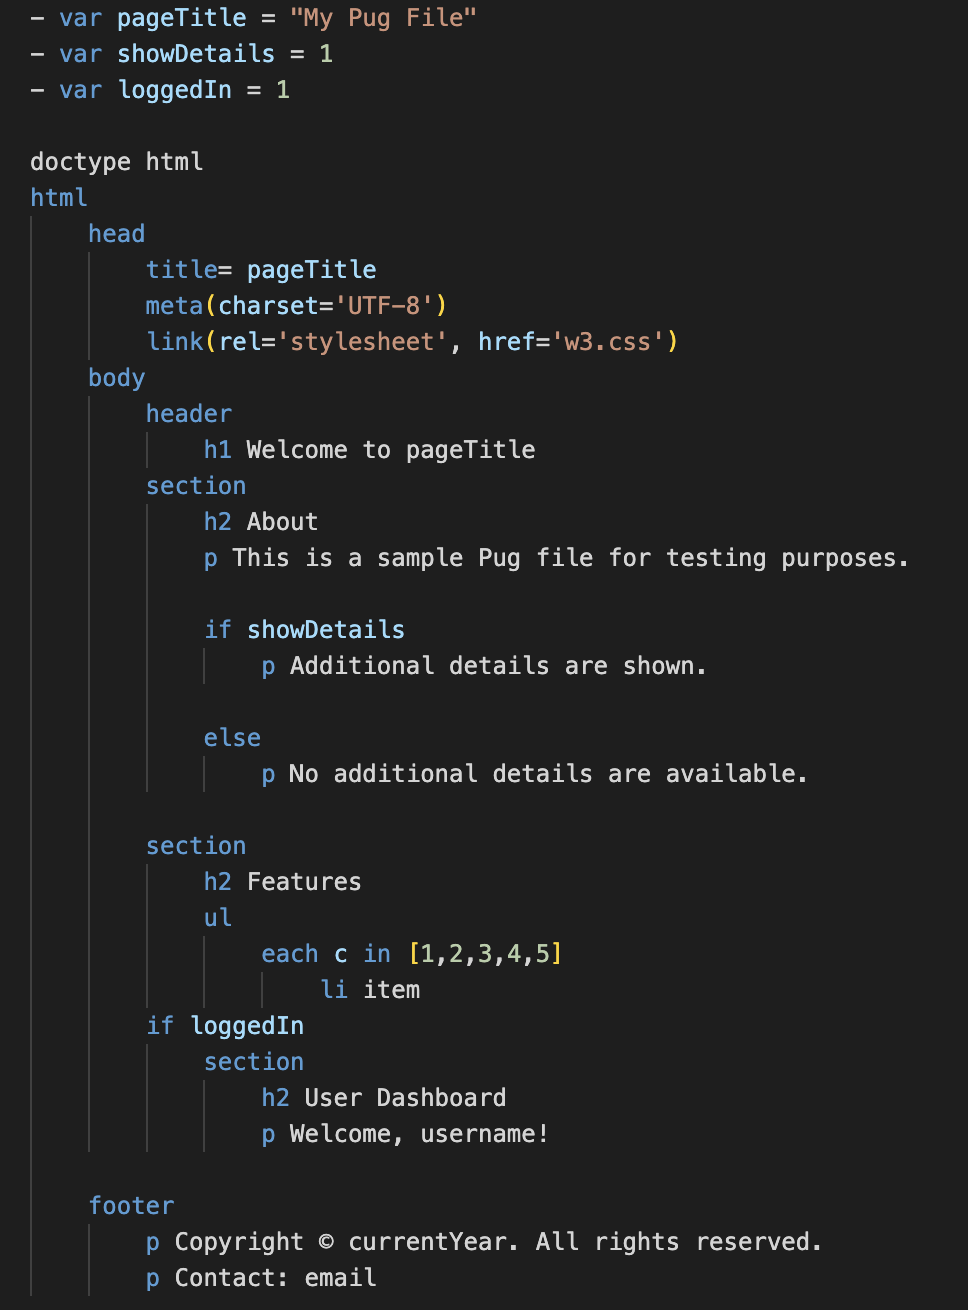
\includegraphics[width=\linewidth]{pug.png}%
  }%
  \hfill
  \subcaptionbox{HTML}[.45\linewidth]{%
    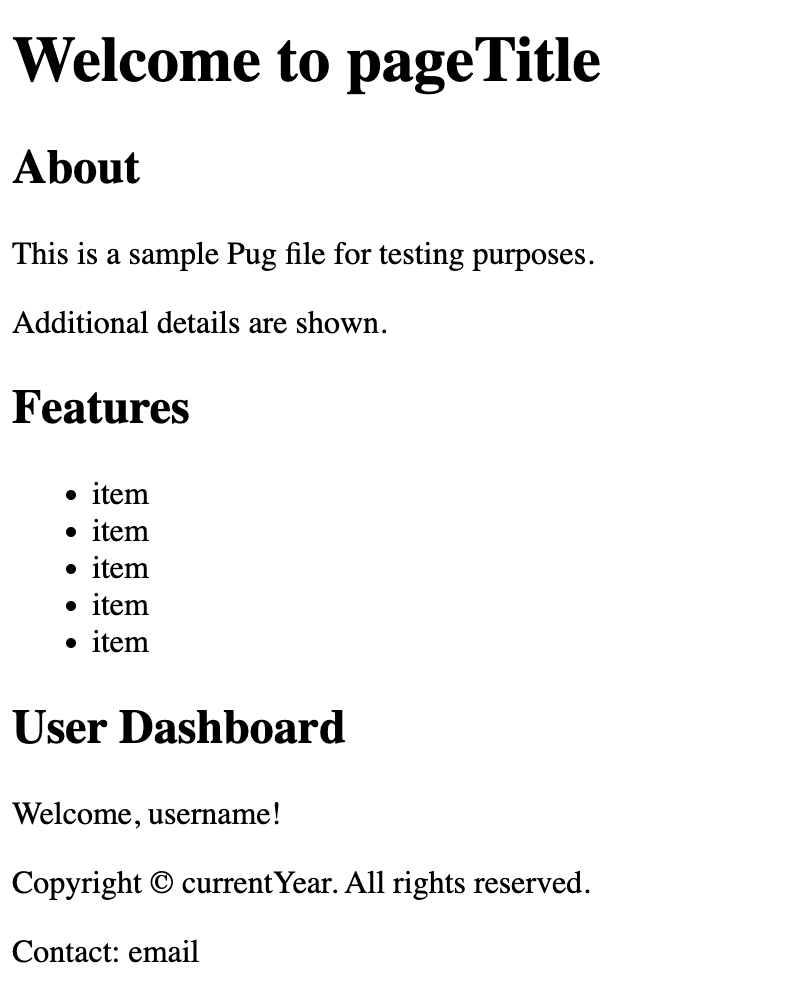
\includegraphics[width=\linewidth]{html.png}%
  }
  }
  \caption{Um dos testes}
\end{figure}

\chapter{Conclusão} \label{concl}
Em suma, o nosso grupo considera que, embora não tenhamos conseguido implementar todas as funcionalidades do \textit{Pug}, conseguimos desenvolver um conversor eficaz de \textit{Pug} para \textit{HTML}, que foi capaz de lidar com os exemplos fornecidos pelo professor, bem como diversas outras funcionalidades. Durante o processo, enfrentamos desafios significativos, mas fomos capazes de superá-los e entregar um produto funcional. Reconhecemos que há espaço para melhorias e expansões futuras, mas estamos satisfeitos com os resultados alcançados até o momento. Através deste projeto, aprofundamos nosso conhecimento de processamento de linguagens e adquirimos habilidades valiosas na implementação de conversores de linguagens. No geral, estamos orgulhosos do nosso trabalho e confiantes de que cumprimos os objetivos propostos, obtendo um resultado satisfatório.

\newpage
%\bibliographystyle{plain} % [1] Numérico pela ordem de citação ou ordem alfabetica
\bibliographystyle{alpha} % [Hen18] abreviação do apelido e data da publicação
%\bibliographystyle{apalike} % (Araujo, 2018) apelido e data da publicação
                             % --para usar este estilo descomente no inicio o comando \usepackage{apalike}

\bibliography{bibLayout} %input do ficheiro de referencias bibliograficas

\end{document} 